\section{Experimental Design}\label{sec:eval-design}
% \begin{figure}
%     \centering
%     \includegraphics[width=\columnwidth]{figures/planner_ops_smol.png}
%     \caption{The Planning Procedure: Step 1: Using the method from \cref{fig:edge_selection}, select edges to try in simulation; Step 2: Try the edges in simulation and save the action that moves the object closest to the goal; Step 3: Execute that edge on the real robot.}\vspace{-15pt}
%     \label{fig:timeline}
% \end{figure}
\begin{figure}
    \centering
    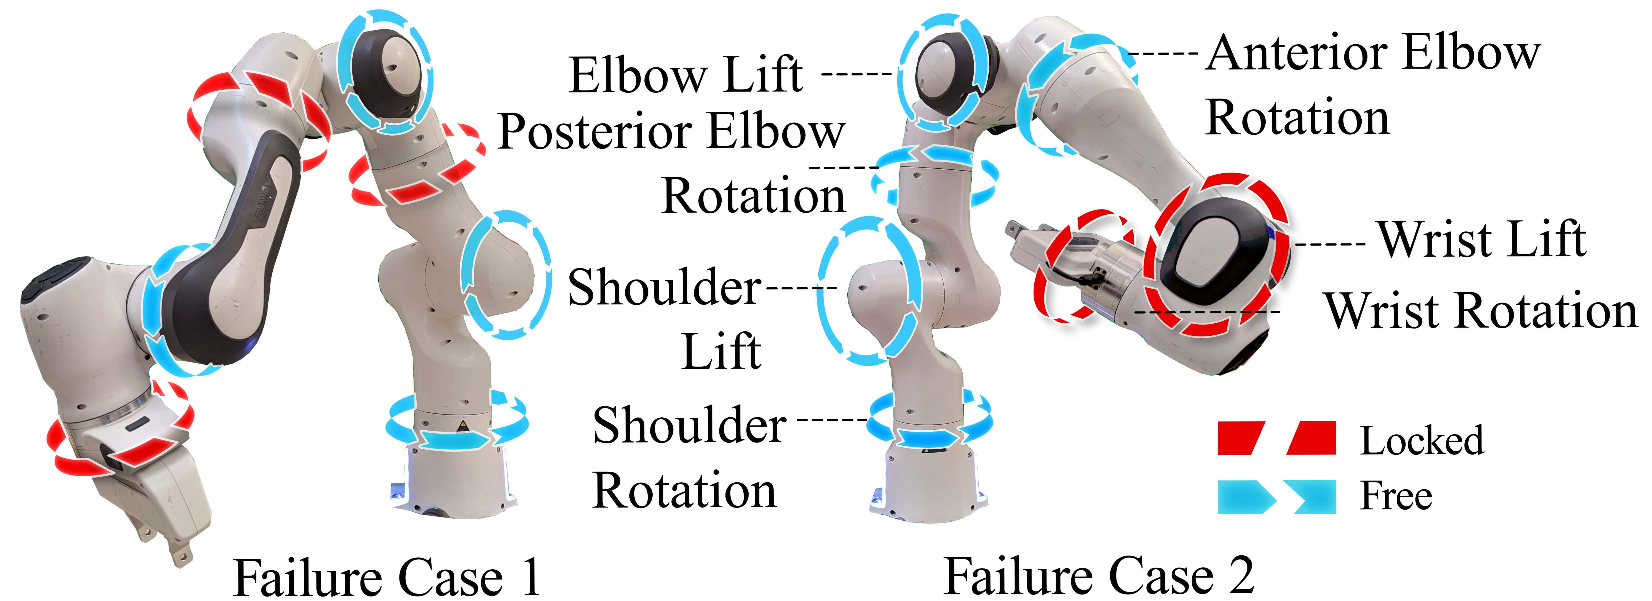
\includegraphics[width=\columnwidth]{figures/Figure_3_update_02b_comp-1.pdf}
    
    \caption{Franka Emika Panda robotic arm with multiple locked joints. The left represents Failure Case 1, with the locked Anterior and Posterior Elbow Rotation and Wrist Rotation joints locked. The right represents Failure Case 2 with locked Wrist Lift and Rotation joints.}
    \label{fig:panda_crippled}
\end{figure}
\begin{figure}
    \centering
    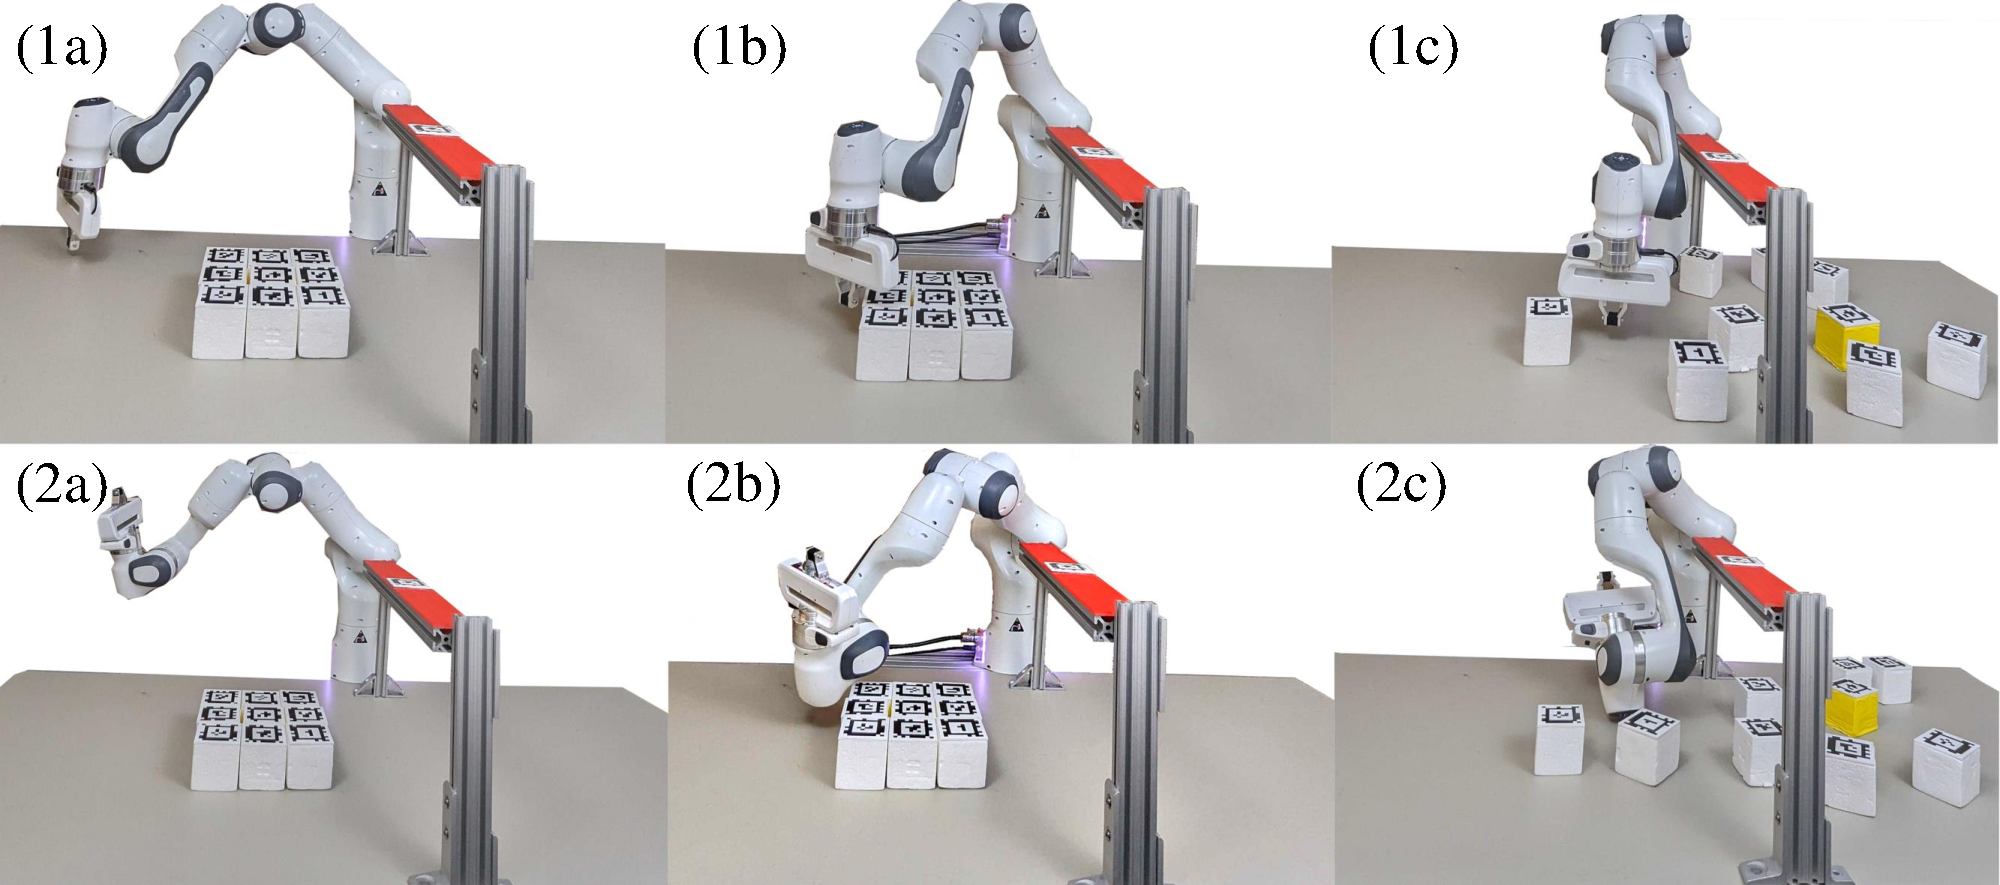
\includegraphics[width=\columnwidth]{figures/action_sequence.pdf}
    
    \caption{This figure presents two action sequences demonstrating the NPM interaction using different robot embodiment areas. The top sequence (1a-c) illustrates the interaction using the end effector, while the bottom sequence (2a-c) shows the interaction utilizing the robot’s whole embodiment. These sequences represent a composite scenario derived from scenarios 2 and 3, providing an illustrative view of the robot’s expanded capabilities.}
    \label{fig:action_example}
\end{figure}
\begin{figure*}
    \centering
    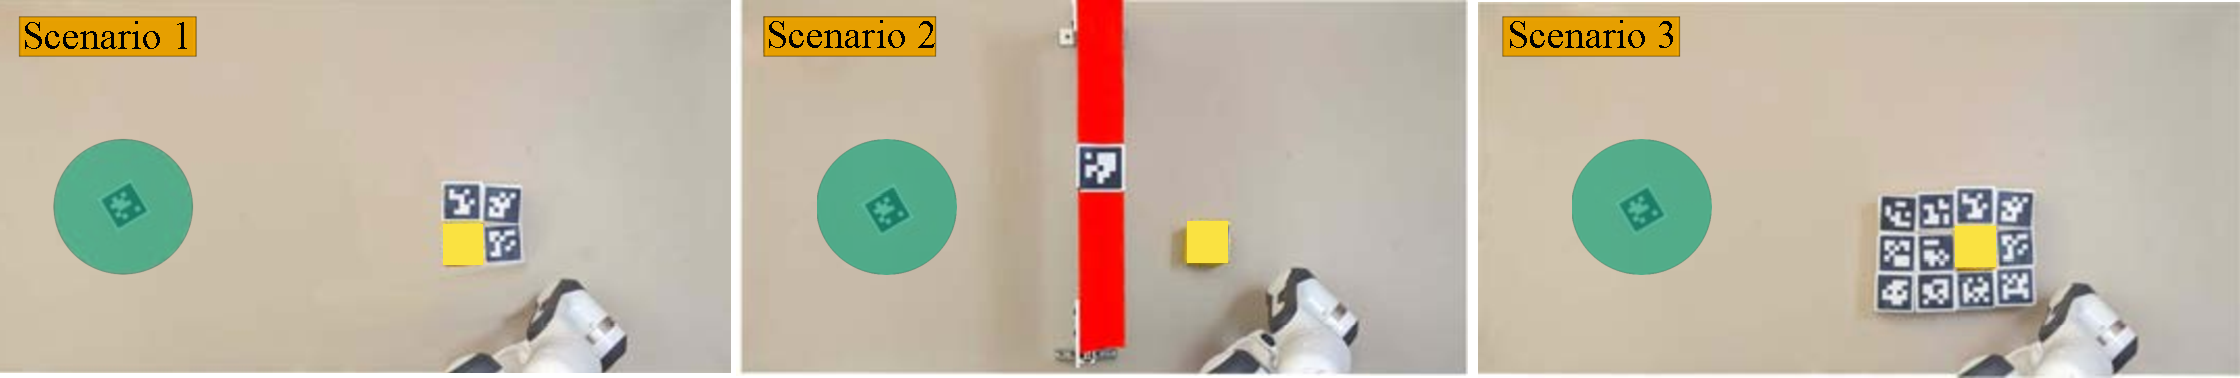
\includegraphics[width=\textwidth]{figures/scenarios-compressed_9.pdf}
    \caption{This figure presents three distinct scenarios tested in the study. Scenario 1 (left) features three movable obstacles (white with fiducial markers) and one target object (yellow). Scenario 2 (center) introduces a tunnel obstacle partitioning the table. Scenario 3 (right) includes 11 movable obstacles and one target object. The green shaded area represents the goal for each Scenario. \vspace{-15pt}}
    \label{fig:scenarios}
\end{figure*}
We test our system in three real-world scenarios with two LMJ cases across three different ablative ASMs. These failure cases, shown in \cref{fig:panda_crippled}, demonstrate two different families of failures that can occur: Case 1 limits the end effector grasping ability to a portion of the reachable area, and Case 2 precludes the use of the end effector in its entirety. Without loss of generality, these two cases represent a subset of the many permutations of faults that can occur due to LMJs. Our results are a quantitative analysis of the planning time, success rate, and reachability improvements resulting from utilizing the robot's whole embodiment combined with NPM actions. Two representative NPM actions are shown in \cref{fig:action_example}.
% \textit{ADAPT-R} enables the robot to complete tasks in these failure cases where prior approaches would fail \cite{xie2021maximizing, porges2021planning}.

We consider two failure cases in our evaluation: 
% The Failure Cases are as follows:
\begin{itemize}
    \item \textbf{Failure Case 1} (\cref{fig:panda_crippled}, left): The first case involves locking three joints: the Posterior Elbow Rotation, Anterior Elbow Rotation, and Wrist Rotation Joints.
    % This limits the robot's PM capability by drastically restricting the set of valid grasp configurations, as reflected by robot's reachable task space area and by limiting the end-effector orientations.
    This limits the graspable area and reduces the range of grasping configurations by coupling the end-effector orientation to the joint configuration.
    \item \textbf{Failure Case 2} (\cref{fig:panda_crippled}, right): In the second case, two joints are locked: the wrist lift and wrist rotation joints. This failure case precludes the use of the end-effector in completing manipulation tasks. This enables us to test the system using exclusively the non-end-effector parts of the robot's embodiment. 
\end{itemize}
The experimental scenarios are presented in \cref{fig:scenarios}. Each scenario involves manipulating the target object (the yellow cube) to the goal location (green area):
\begin{itemize}
    \item \textbf{Scenario 1} (\cref{fig:scenarios}, left): This scenario has three movable obstacles and one target object. This scenario is motivated by the need to be able to manipulate in cluttered environments that hinder direct access to the target object. 
     \item \textbf{Scenario 2} (\cref{fig:scenarios}, center): The second scenario has a tunnel obstacle in the middle, partitioning the two halves of the table. This scenario is motivated by the need to perform dexterous manipulation while maneuvering around environmental obstacles.
    \item \textbf{Scenario 3} (\cref{fig:scenarios}, right): There are 11 movable obstacles and one target object. This scenario allows us to explore the utility of our planner in the presence of increased object-obstacle interactions.
\end{itemize}

% We conduct an ablative study across multiple Pick Action Methods:
% \begin{itemize}
%     \item \textbf{Greedy}: The Greedy action selection method utilizes our sim-in-the-loop planner to find an edge that moves the target object toward the goal. Of all the edges that intersect the object, it selects the first action that moves the target towards the goal in the simulator.
%     \item \textbf{Random}: The Random action selection method finds all the edges that intersect the object and picks one randomly.
%     \item \textbf{Cautious}: The Cautious action selection will sample five percent of the edges that intersect the object and score them based on how close the target object is to the goal after simulating the selected actions. It will command the highest-scored edge for the real robot.
% \end{itemize}

% because our planner’s primary purpose is to complete tasks under failure.
To comprehensively understand how NPM abilities expand the robot's task space, we conduct the reachability analysis in \cref{sec:reach_anls}. In \cref{sec:planner_eval}, we show the effectiveness of our system across the three scenarios shown in \cref{fig:scenarios}, for the two failure cases described in \cref{fig:panda_crippled}, using the three Action Selection Mechanisms described in \cref{sec:methods-planning} over a total of 267 trials. This analysis shows the limitations of grasping-only actions and demonstrates the improvements brought about by NPM abilities.
% to show the limits in the task space of grasping-only actions and the improvements enabled through NPM abilities.
% Below, we present our findings on the increase in reachability for a given task plane in \cref{sec:reach_anls} and an analysis of our experimental results in testing \textit{ADAPT-R} in \cref{sec:planner_eval}. 
Through these results, we seek to verify two hypotheses:
% \begin{itemize}
%     \item[\textbf{H.1}] Combining NPM abilities with whole-body interaction increases the manipulable area of a robot arm experiencing LMJs.
%     \item[\textbf{H.2}] Implementing NPM abilities can increase the success of a robot conducting tabletop manipulation tasks.
% \end{itemize}
\begin{itemize}
    \item[\textbf{H.1}] When experiencing LMJs that limit or disallow the use of the end-effector, whole-body NPM abilities increase the manipulable area of a robot manipulator.
    \item[\textbf{H.2}] When experiencing LMJs that limit or disallow the use of the end-effector, whole-body NPM abilities can increase the success rate of a robot conducting tabletop manipulation tasks.
\end{itemize}


\section{Experimental Results}\label{sec:eval}

\subsection{Reachability and Manipulation Capability Analysis}\label{sec:reach_anls}
Relying solely on the end effector renders the robot ineffectual in failure cases that severely or entirely limit its use.
NPM abilities and the capability to interact with the environment using the whole embodiment allow for increased robot manipulable area. To study this, we analyzed the robot's manipulable area and capabilities over the task space of the evaluation scenarios.
The manipulable area is found through the method presented in \cref{sec:methods-reachability}.

\begin{table}[]
\centering
\begin{tabular}{@{}cccc@{}}
\toprule
\textit{\textbf{Failure Case}} & \textit{\textbf{Ability}} & \textit{\textbf{Area (m$^2$)}} & \textit{\textbf{Change in Reachable Area}}\\ \midrule
\textit{No Failure} & \textbf{NPM+PM} & \textbf{0.92} & Datum \\ %\midrule \textit{No Failure}
 & PM     & 0.85 & -$8\%$ \\ \midrule
\textit{1}       & \textbf{NPM+PM} & \textbf{0.85} & \textbf{-8\%} \\ %\midrule % 0.8521 \textit{1} 
      & PM     & 0.62 & -$33\%$ \\ \midrule
\textit{2}       & \textbf{NPM+PM} & \textbf{0.73} & \textbf{-21\%}  \\ %\midrule \textit{2}  
     & PM     & 0 & -$100\%$      \\ \bottomrule
\end{tabular}
\caption{Reachability Data \vspace{-15pt}}
\label{tab:reachability}
\end{table}

The nominal full-dexterity manipulable area is 0.85 $m^2$; the use of NPM increases this area to 108\% of nominal (\cref{tab:reachability}, rows 1 and 2). The manipulable area in the first failure case is severely limited by the inability to control the end-effector's orientation and task space movements in the z-axis when the end-effector is closer to the robot's base. When using NPM actions, the robot maintains 92\% of the reachable area compared to 67\% when using PM actions only (\cref{tab:reachability}, rows 3 \& 4). Since Failure Case 2 precludes the use of the end-effector, the PM-only reachable area is eliminated. However, using NPM actions, the reachable area is only reduced by 21\% (\cref{tab:reachability}, rows 5 \& 6).

The results show that \textbf{in failure modes that disallow or limit the use of the end effector, utilizing the whole body of the robot with NPM actions significantly expands the area of the robot's reachable space, supporting H.1.}

\begin{figure*}
    \centering
    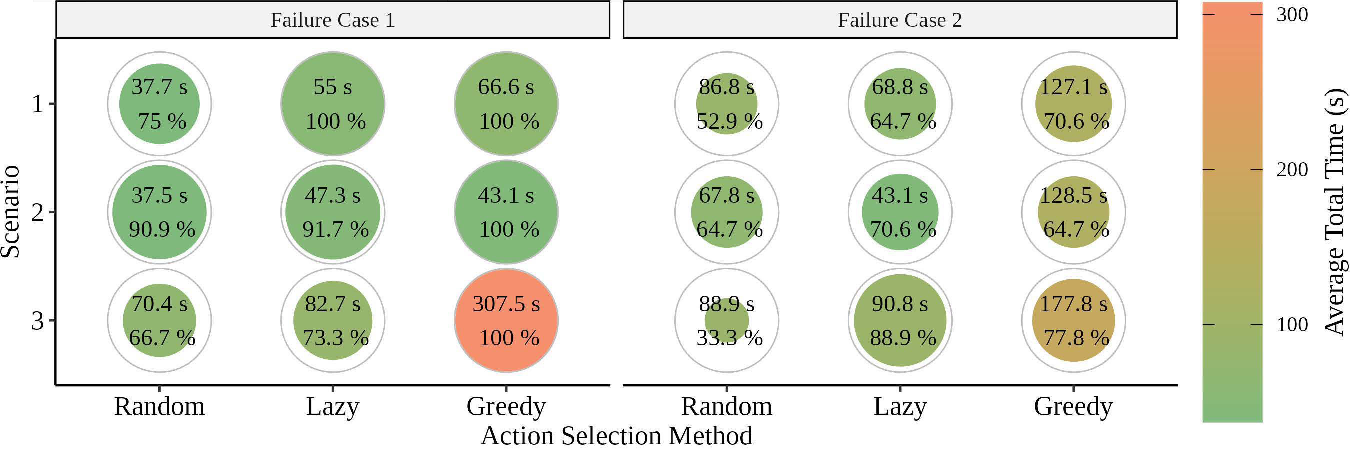
\includegraphics[width=\textwidth]{figures/both_flipped_5.pdf}
    \caption{Comparative performance of Action Selection Methods across the Failure Cases. The color intensity of each circle indicates the task time, with green colors representing lower times and red colors indicating higher times. The size of each circle represents the success rate, with larger circles denoting higher rates.\vspace{-10pt}}
    \label{fig:bubble}
\end{figure*}
\begin{figure*}
    \centering
    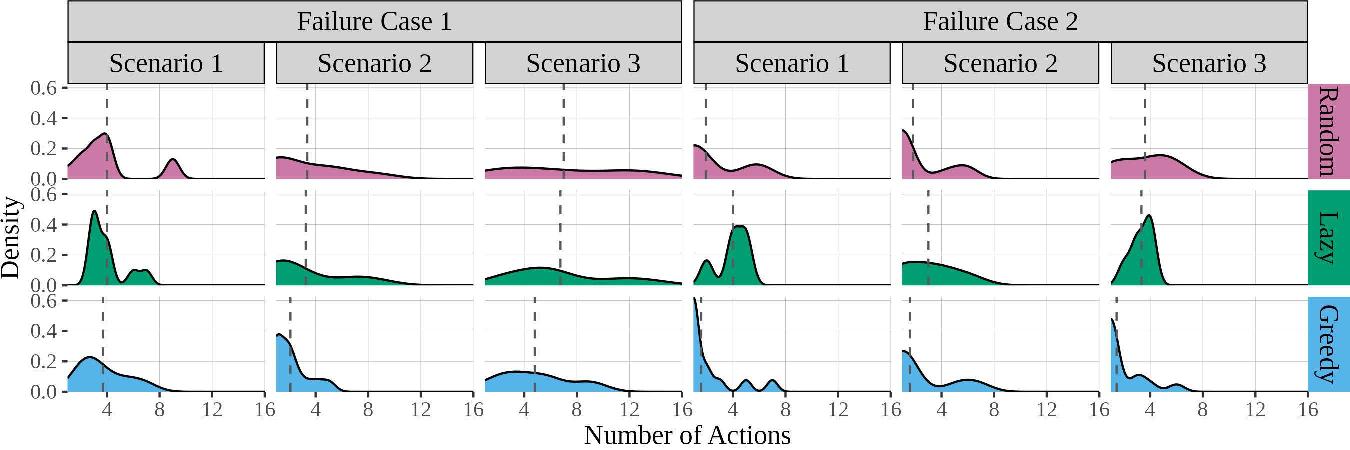
\includegraphics[width=\textwidth]{figures/shoulder_wrist_actions_comp_3.pdf}
    \caption{The distribution of actions required to complete different scenarios for each failure case using the action selection methods. Each graph represents a scenario under a specific failure case, with the x-axis indicating the number of actions and the y-axis representing the density across all trials. \vspace{-10pt}}
    \label{fig:shoulder-actions-comp}
\end{figure*}
\subsection{Real-world Manipulation Results}\label{sec:planner_eval}
% \begin{table}[]
% \centering
% \begin{tabular}{ccccc}
% \hline
% \textbf{}       & \multicolumn{3}{c}{\textbf{Task Time {[}seconds{]}}}                        & \textbf{Success Rate} \\ \hline
% \textbf{Planner}  & \textbf{S1} & \textbf{S2} & \textbf{S3} & \textbf{S1-S3} \\
% \textbf{Lazy} & \textit{\textbf{69.53}} & \textit{\textbf{62.25}} & \textit{\textbf{85.92}} &\textit{ \textbf{75.0\%}}       \\
% \textbf{greedy} & 146.23      & 130.46      & 127.53      & 61.2\%         \\
% \textbf{Random}   & 97.37       & 74.26       & 94.64       & 60.0\%         \\ \hline
% \end{tabular}
% \caption{Task Times For Failure Case 2}
% \label{tab:task-times-fc2}
% \end{table}


\cref{fig:bubble} shows the average total task time and success rates across Scenarios 1-3, Failure Cases 1 and 2, and the Random, Lazy, and Greedy ASMs. Across the ASMs, we see a trend of the Greedy method taking the longest, up to 307.5s, and the Random method taking the shortest time, as low as 37.5s, to complete the task, with the Lazy method roughly falling in between, at 47.3s-82.7s. This is expected because when averaged over all scenarios, the Greedy edge selection takes more time to plan than the other methods. Regarding the success rate, we see a clear trend in Failure Case 1, where the Greedy edge selection method has a 100\% success rate across all scenarios, and the Random edge selection has the lowest success rate. The Lazy edge selection has a success rate that, at best, matches the Greedy selection method at 100\% and, at worst, is better than the Random selection method, at 73.3\% vs. 66.7\% for Scenario 3. However, for Failure Case 2, no clear trend for the success rate occurs. Overall, the Lazy selection case is successful in scenarios 2 and 3, while the other two ASMs tend to have poorer results, except in scenario 1 for the Greedy ASM at 70.6\%. These results come from the combination of the inherent stochastic nature of the NPM interactions multiplied by the decreased sim-to-real accuracy of our sim-in-the-loop planner when interacting with areas of the robot that are not the end effector, as this failure case requires. This can partly be explained by the slight differences between our simulated collision meshes and the real robot embodiment.

% \begin{table}[]
% \centering
% \resizebox{\columnwidth}{!}{%
% \begin{tabular}{@{}ccccccc@{}}
% \toprule
%                   & \multicolumn{6}{c}{\textbf{Execution Time}} \\ \midrule
% \textbf{}                                              & \multicolumn{3}{c}{\textbf{Failure Case 1}} & \multicolumn{3}{c}{\textbf{Failure Case 2}} \\
% \multicolumn{1}{l}{\textbf{Selection Method}} & \textbf{Scenario 1}    & \textbf{Scenario 2}   & \textbf{Scenario 3}   & \textbf{Scenario 1}    & \textbf{Scenario 2}   & \textbf{Scenario 3}   \\
% \textbf{greedy} & 26.7  & 11.7  & 20.1  & 10.5  & 12.3 & 13.0 \\
% \textbf{Lazy}   & 27.1  & 19.7  & 21.2  & 13.7  & 10.1 & 21.1 \\
% \textbf{Random}   & 25.2  & 16.1  & 15.1  & 9.29  & 11.1 & 18.8 \\ \bottomrule
% \end{tabular}%
% }
% \caption{Execution Time Summary}
% \label{tab:exec-times}
% \end{table}

% \begin{figure*}
%     \centering
%     \includegraphics[width=\textwidth]{figures/time_comparison.pdf}
%     \caption{Comparison of Planning and Execution times across the Failure Cases and the Edge Selection Methods averaged over all Scenarios \gm{TODO: Fix Font and Text Size | Should this just be replaced with a table of averages?}}
%     \label{fig:time-comp}
% \end{figure*}



In \cref{fig:shoulder-actions-comp}, we see the distribution of the number of actions needed to complete a scenario successfully for the three different action selection methods. Across both failure cases and all scenarios, we see a trend of the Greedy ASM requiring, on average, the fewest actions to complete the given task. This strongly supports the usefulness of including a simulator in planning to inform the best action. When comparing the Lazy and Random ASMs, we see that the Random approach usually has a flatter or wider multi-peak distribution. This is expected as the Random approach can complete the task in one action or require many actions. The Lazy ASM is a balance between the two extremes. In Failure Case 1, the average number of actions sits between the Greedy and Random ASMs. In contrast, in Failure Case 2, we see the weakness of its one-shot approach, taking one to two more actions, on average, to complete than the Random or Greedy approach. Still, there is less deviation than the Random approach, with a shorter tail on the higher end of the actions needed.

Overall, our data shows a new and unique ability to conduct manipulation tasks while experiencing LMJs that restrict the robot's capability to manipulate using traditional pick-and-place approaches. Our sim-in-the-loop planner improved the robot's ability to conduct these tasks by looping in a physics model to our NPM actions. We demonstrated that a balanced approach of speed and simulation accuracy can complete our manipulation scenarios well. We have \textbf{shown that while experiencing LMJs, our approach can unlock the capability of robotic manipulators to conduct tabletop manipulation successfully, supporting H.2.}

% \subsection{Planner Evaluation}\label{sec:planner_eval}
% \begin{figure*}
%     \centering
%     \includegraphics[width=0.95\textwidth]{figures/planner_eval_smol.pdf}
%     \caption{Representative Scenario Solutions. Each image represents how the robot solved the scenario for each failure case. The colored lines are the motions of the robot end effector tip, with the color representing the manipulability of the robot. For each, the yellow boxes represent the target object or objects. The black outlined boxes in the first scenario represent the obstacles. For the first two scenarios, the black lines represent the motion of the target object. For visual simplicity, the final scenario only shows the final positions of the target objects.}
%     \label{fig:planner_ops}\vspace{-15pt}
% \end{figure*}



\subsubsection{Behavior of the Planner} 
We analyze the planner's quality through its behavior in the two failure scenarios through an analysis of the robot's actions to complete the tasks. For some of the cases, we will discuss two examples, one good and one bad, to understand better how the planner can be limited. In each of the cases, in \cref{fig:planner_ops}, we see the path the target object or objects took, the final position of any obstacles, and the path of the robot's end effector tip colored by the manipulability of the arm through the path.

\textbf{Failure Case 1}: In Test Scenario 1, we see the error in the sim-to-real action execution. The planner commands several actions, but the actions executed on the robot fail to move the target object from its initial position. During that time, the robot rearranges the obstacle objects significantly. Once the robot moves the target object initially, the arm is then able to execute a strong action and move the target object deep into the goal region.

In Test Scenario 2, we see the robot initially staying clear of the tunnel and then poking its end effector under the tunnel to move the object into the goal region outside of its reachable range.

Test Scenario 3 highlighted the challenges of manipulating objects near the edge of the robot's working space. Many of the actions here didn't go smoothly and had low manipulability throughout, causing significant discrepancies between what the simulation predicted and what the real robot could achieve. As a result, it took a total of eleven actions to move all four objects to the target region successfully.

\textbf{Failure Case 2}: In Test Scenario 1, we see that the scenario was completed in two actions, with each action moving the block in the direction of the goal. This represents the best-case scenario of the planner, where the sim-to-real system has very small errors and will move the object consistently with the goal of shrinking the gap to the target area. 

In Test Scenario 2,  we see how errors in the sim-to-real system can lower the performance of the planner. For this scenario, the planner commanded the robot to execute six actions. In the simulation-in-the-loop, these six actions interact with the target object and move it towards the goal. However, we only see the target object move five steps from the initial position to the goal; thus, the robot misses touching the target object entirely. There was only minimal contact between the arm and the object for two of the actions, causing only small movements. 

In Test Scenario 3, the robot efficiently moves three of the four target objects to the goal region with just two actions. However, those first two motions knock the fourth object away from the robot to an area with consistently lower manipulability. This means the planner commands four actions before a quality contact is made and the target reaches the goal.
\subsubsection{Strengths}
% greedy approach can lead to quick solutions and does not require optimization tuning 
% multi object manipulation
% dynamic interaction point -- no concern about which point on the robot an object touches, means the planner can make both sweeping actions across multiple object simultaneously and delicately control a single object
One of the key advantages of the planner is its efficient nature, thanks to a greedy approach that prioritizes quick solutions without the need for extensive optimization tuning. This quality expedites the planning process and simplifies the implementation of complex tasks. Furthermore, the planner excels in multi-object manipulation scenarios, where it can seamlessly coordinate the robot arm's movements to interact with multiple objects simultaneously. Its ability to manage dynamic interaction areas, irrespective of which part of the robot touches an object, allows for sweeping actions across multiple objects and delicate, precise control when dealing with a single object. This flexibility and adaptability make the task and motion planner a valuable tool for a wide range of robotic applications, where speed, versatility, and precision are paramount.

\subsubsection{Weaknesses}
% Greedy approach can lead to suboptimal actions and long plans
% scoring method for edge selection is too simple, can not remember what makes a 'good' action so repeatability is bad
% Sim to real can be very wrong
% sim in loop can increase planning times
% imperfect dynamics model for edge generation leads to even more error between simulation actions and real actions
One notable limitation is the use of a greedy approach, which, in certain scenarios, may result in suboptimal actions and lead to longer less efficient plans. Additionally, the planner relies on a relatively simple scoring method for edge selection, which lacks the ability to remember what constitutes a `good' action, resulting in poor repeatability. The challenge of sim-to-real transition can also pose difficulties, as the planner may struggle to accurately replicate real-world actions from simulations, leading to discrepancies and errors. Moreover, incorporating simulation-in-loop can increase planning times, potentially affecting real-time applications negatively. Lastly, the imperfect dynamics model used for edge generation can further exacerbate the gap between simulated actions and real-world outcomes. Despite these weaknesses, the planner's advantages make it a valuable tool for various robotic tasks when used judiciously and with consideration of these limitations.

These experiments show that \textbf{our approach successfully utilizes the kinodynamic map and the increased reachability of the robot arm to complete manipulation tasks in the face of LMJ through the use of non-prehensile movements, supporting H.2.}



